\documentclass[a4paper]{article}
\usepackage[latin1]{inputenc} 
\usepackage[T1]{fontenc}
\usepackage{graphicx}
\usepackage{lmodern}          
\usepackage[colorlinks=true, urlcolor=blue, breaklinks, pagebackref, citebordercolor={0 0 0}, filebordercolor={0 0 0}, linkbordercolor={0 0 0}, pagebordercolor={0 0 0}, runbordercolor={0 0 0}, urlbordercolor={0 0 0}, pdfborder={0 0 0}]{hyperref} 
%\usepackage[ngerman]{babel}
\usepackage{listings}             % Include the listings-package
\usepackage{xcolor}
\lstset{language=bash, columns=fullflexible, extendedchars=false, backgroundcolor=\color{lightgray}, breaklines=true}

\title{\textbf{Fafoom}\\Flexible algorithm for optimization of molecules \\ 2.0.0}
%\title{Fafoom -Flexible algorithm for optimization of molecules}

\begin{document}
\maketitle

\tableofcontents
\newpage

\section{An overview of Fafoom}

Fafoom is a Python module for optimization of organic molecules primarily intended to work with \href{https://doi.org/10.1021/acs.jcim.5b00243}{FHI-aims} (Fritz Haber Institute ab initio molecular simulations package). 
Fafoom can be utilized for, e.g., performing  a genetic algorithm (GA) search for molecules. The genetic operations (crossover and mutation) explore the fitness function (energy) by changing the degrees of freedom of the molecule. Three sorts of degrees of freedom are currently implemented: torsions, \textit{cis/trans} bonds and pyranose ring configurations. Further, user-defined degrees of freedom can be implemented. Fafoom:
\begin{itemize}
\item initializes the molecule from a SMILES code
\item performs the global search on user-curated selection of degrees of freedom and performs local optimization based on full relaxation of Cartesian coordinates
\item uses for the local optimization an external software that can be easily exchanged
\item is distributed under GNU Lesser General Public License 
\end{itemize}

Fafoom uses eV as a unit for energy. If the utilized software outputs energy in different units, the value is converted to eV after completed local optimization.

\section{Requirements}

For the python module:
\begin{itemize}
\item Python (used for testing: 2.7.6)
\item Numpy (used for testing: 1.8.2)
\item RDKit (used for testing: Release\_2015\_03\_1)
\end{itemize} 
For the first-principles methods:
\begin{itemize}
\item (recommended) FHI-aims (Fritz Haber Institute ab initio molecular simulations package)
\item (alternative) NWChem (NWChem: Open Source High-Performance Computational Chemistry)
\item (alternative) ORCA (An ab initio, DFT and semiempirical SCF-MO package). 

\end{itemize} 

\section{Installation}

\begin{enumerate}
\item Clone the fafoom repository
\begin{verbatim}
git clone https://github.com/adrianasupady/fafoom
\end{verbatim}
or download and unzip the version from :
 \begin{verbatim}
https://github.com/adrianasupady/fafoom/releases
\end{verbatim}
\item Add the fafoom directory to your PYTHONPATH
\item Import the module in python
\begin{verbatim}
import fafoom
\end{verbatim}
\end{enumerate}

\section{Module overview}


\begin{figure}[h!]
  \caption{Flexible algorithm for optimization of molecules Fafoom:  Module overview}
  \centering
    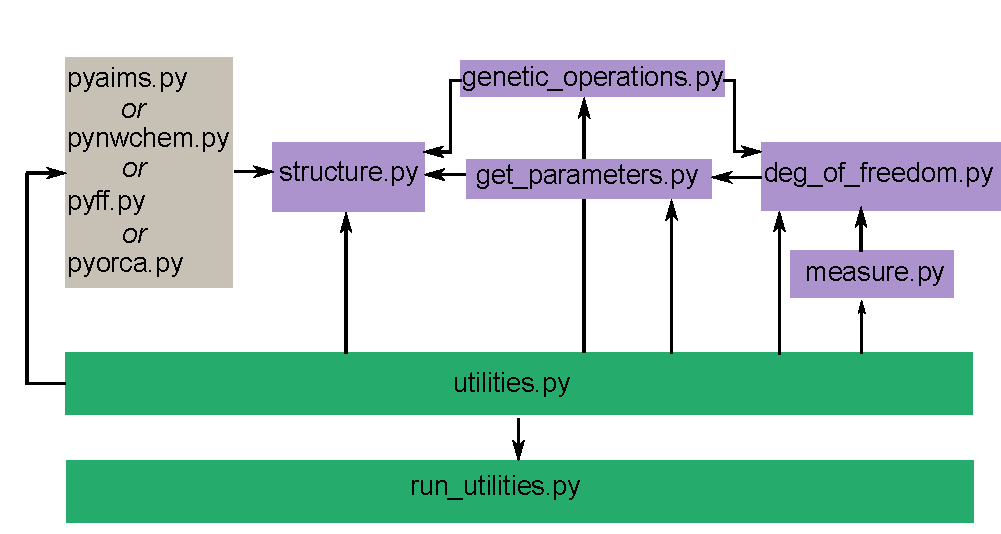
\includegraphics[width=1.0\textwidth]{fafoom_module_overview.pdf}
\end{figure}

\begin{itemize}
\item \textit{structure.py} - the core module of the package, defines two classes: (i) \textbf{MoleculeDescription} that takes care of initializing the molecule and the attributes, that are shared between different 3D structures and should never change their values, i.e. number of atoms or number and location of the user-defined degrees of freedom and (ii) \textbf{Structure} that allows for generating valid and unique 3D structures, calling the external optimizer or genetic operators; further, it takes care of the varying attributes, e.g. the sdf string or values of the degrees of freedom. 

\item \textit{get\_parameters.py} - this module is responsible for obtaining the permanent attributes. It also serves as a link between the \textit{structure.py} and the \textit{deg\_of\_freedom.py} module. 

\item \textit{deg\_of\_freedom.py} - this module defines a separate class for each type of degree of freedoms. The methods of the classes allow for finding the degrees of freedom, assigning, mutating and updating their values as well as generating corresponding sdf strings.

\item \textit{measure.py} - collection of methods for measuring and setting the values of the degrees of freedom

\item \textit{genetic\_operations.py} - collection of genetic operations needed to perform a genetic algorithm

\item \textit{pyaims.py} - wrapper for the FHI-aims simulation package; takes care of performing the local optimization and retrieving and storing the results

\item \textit{pynwchem.py} - wrapper for NWChem

\item \textit{pyorca.py} - wrapper for ORCA

\item \textit{pyff.py} - wrapper for force field calculations performed with RDKit

\item \textit{utilities.py} - collection of diverse help functions: vector operations, conversions between chemical formats, writing to files etc.

\item \textit{run\_utilities.py} - collection of functions that can be used for performing a genetic algorithm run; i.e detecting the variant of the calculation or checking for convergence

\end{itemize}


\section{Getting started}

The fafoom package can be utilized to perform genetic algorithm searches with a selected software for local optimization of the 3D structures. The parameter file needs to define the provider of the energy function to be used ("FHI-aims", "ORCA" or "NWChem" for first principles, "RDKit" for force fields). Depending on the selected software, further keywords need to be specified  (Figure~\ref{Fig:parameters}). The universal syntax for the execution of the runs:

\begin{verbatim}
python ga.py parameter_file
\end{verbatim}

\noindent
Example parameter files are provided together with Fafoom and allow for performing a GA search for alanine dipeptide. Note that the parameter file is divided into three mandatory sections: \textbf{Molecule}, \textbf{GA settings} and \textbf{Run settings}.  To start a test force-field GA search execute:
\begin{verbatim}
python ga.py parameters_ff.txt
\end{verbatim}
\noindent
The details about the run will be written to the \texttt{output.txt}. Just after the start, the \texttt{output.txt} should look like:
\begin{verbatim}
Local optimization will be performed with RDKit.
Number of atoms: 22
Number of bonds: 21
Number of identified torsion: 2
Identified torsion: [(1, 3, 4, 9), (7, 5, 4, 9)]
Number of identified cistrans: 2
Identified cistrans: [(0, 1, 3, 4), (4, 5, 7, 8)]
...
\end{verbatim}
\noindent
The first lines of the \texttt{output.txt} file allow the user to review the search setup. The molecule is build accordingly to the \textbf{SMILES} code that can be obtained from chemistry databases. Alternatively, e.g. Open Babel can be used to create the \textbf{SMILES} from the molecular 3D Cartesian coordinates. For the recognition of degrees of freedom, \textbf{SMARTS} that define molecular patterns are used.\footnote{For more information consult:\href{http://www.daylight.com/dayhtml_tutorials/index.html}{http://www.daylight.com/dayhtml\_tutorials/index.html}}

In the alanine dipeptide case four dihedral angles are identified. A dihedral angle is represented as a tuple of four atom indicies (note that RDKit counts the atoms starting from 0). The \textbf{SMARTS} pattern definitions (smarts\_torsion, smarts\_cistrans and filter\_smarts\_torsion) are adjusted so that the peptide bond is treated in the \textit{cis/trans} mode. Thus, only two of the identified dihedral angles will be treated as fully rotatable. The remaining two will be restricted to adopt only two values: 0$^{\circ}$ and 180$^{\circ}$.
It is advisable to verify if the atom indices and the assigned types match the expectations.


\begin{figure}
  \footnotesize
  \begin{verbatim}  
[Molecule]

smiles= "CC(=O)N[C@H](C(=O)NC)C"
optimize_torsion= True
optimize_cistrans= True
smarts_torsion= "[C,N,O]~[!$(*#*)&!D1]-&!@[!$(*#*)&!D1]~[C,N,O]"
smarts_cistrans= "C~[$(C=O)]-[$(NC)]~[C]"
filter_smarts_torsion= "C~[$(C=O)]-[$(NC)]~[C]"
rmsd_type= "cartesian"
distance_cutoff_1= 1.2
distance_cutoff_2= 2.15
rmsd_cutoff_uniq= 0.25
chiral=True

[GA settings]

energy_var= 0.001
selection= "roulette_wheel"
fitness_sum_limit= 1.2
popsize= 10
prob_for_crossing= 0.95
prob_for_mut_cistrans= 0.6
prob_for_mut_torsion= 0.8
max_mutations_cistrans= 1
max_mutations_torsion= 2


[Run settings]

max_iter= 30
iter_limit_conv= 20
energy_diff_conv= 0.001 

### FHI-aims
energy_function= "FHI-aims"
sourcedir= "adds"
aims_call= "mpirun -n 4  aims.071914_7.scalapack.mpi.x"

### for NWChem:
energy_function= "NWChem"
functional= "xpbe96" 
basis_set= "STO-6G"
nwchem_call= "mpirun -n 4 nwchem"

### RDKit:
energy_function= "ff"
force_field= "mmff94"
steps= 1000
force_tol= 1e-04
energy_tol= 1e-06

### ORCA:
energy_function= "orca"
commandline= "opt pbe nopop miniprint"
chargemult= "0 1"
optsteps = 200
nprocs= 4
memory= 4000
orca_call= "/full/path/to/orca/"


  \end{verbatim}
  \normalsize
  \vspace*{-4.0ex}
\caption{\label{Fig:parameters}
	  \textbf{\large{parameters.txt}}
 }
\end{figure}


\noindent
For the meaning of the parameters and available options get familiar with section \textbf{Keywords}.
\noindent
Backup text files for the restart are created after each completed iteration. 



\subsection{GA with FHI-aims}
Before running the algorithm, a a directory containing the \texttt{control.in} file that will be used for the FHI-aims calculations needs to be created. During the run, one new directory will be created for each FHI-aims calculation. If needed, take a look at pyaims.py and adjust it for your needs.
\subsection{GA with NWChem}
If you want to modify the geometry optimization settings, adjust the pynwchem.py file. 
\subsection{GA with ORCA} 
Details concerning the geometry optimization with ORCA can be found in following chapters of the ORCA manual: \textbf{Running Typical Calculations: Geometry Optimizations, Surface Scans, Transition States, MECPs} (5.2) and \textbf{Detailed Documentation: Geometry Optimization} (6.13).

\subsection{Restart}
The algorithm can be restarted if at least one generation has been successfully completed. The information transfer happens via the backup files that are generated after a completed generation. During the restart, the population and the blacklist are rebuild. If all necessary backup files are present, the restart can be started directly with:

\begin{verbatim}
python ga.py parameter_file
\end{verbatim}





\section{Keywords}

This section lists all recognized keywords. Some of them are depended on each other and on the selected system, e.g. 'optimize\_cistrans' will cause no effect unused is no \textit{cis/trans} bonds are found. The absolutely required keywords are underlined. 
\vspace{10pt}

\noindent
\textbf{\large{Molecule settings}}

\begin{itemize}

	
    \item{\underline{\textbf{\large{smiles}}}}
	
Simplified one-line notation (SMILES) of the compound you want to perform the search for.  
	\item{\textbf{optimize\_torsion}}, default = True 

Set True, if you want the torsions of be among the optimized degrees of freedom.

	\item{\textbf{optimize\_cistrans}}, default = False

Set to True, if you want the \textit{cis/trans} bonds of be among the optimized degrees of freedom.

	\item{\textbf{optimize\_pyranosering}}, default = False

Set to True, if you want the pyranosering bonds of be among the optimized degrees of freedom.

	\item{\textbf{smarts\_torsion}}, default="[*]$\sim$[!\$(*\#*)\&!D1]-\&!@[!\$(*\#*)\&!D1]$\sim$[*]"

Pattern for matching torsions. The default value will match the following pattern: (any atom)(any bond)(a non-terminal atom that is not triply connected)(single bond)(a non-ring and non-terminal atom, that is not triply connected)(any bond)(any atom). 

	\item{\textbf{smarts\_cistrans}}

Pattern for matching \textit{cis/trans} bonds. 

	\item{\textbf{filter\_smart\_torsion}}

The pattern defined here will be used to match torsions you want to ignore. 

	\item{\textbf{list\_of\_torsion}, \textbf{list\_of\_cistrans}, \textbf{list\_of\_pyranosering}}

If you know the positions of torsions/ \textit{cis/trans} bonds/ pyranoserings to be optimized, you can pass them directly as a list of tuples with 4 atoms each. The numbering is consistent with the numbering of the atoms in the SMILES string.\footnote{The first atom in the SMILES has the index 0. Hydrogen atoms don't get a number first, but only after adding all hydrogen atoms to the molecule.}

	\item{\textbf{distance\_cutoff\_1}}, default = 1.3 \AA
	
Parameter for the geometry check. If two non-bonded atoms 	are closer to each other than \textbf{distance\_cutoff\_1} (\AA) the structure will be rejected. 


\item{\textbf{distance\_cutoff\_2}}, default = 2.15 \AA
	
Parameter for the geometry check. If two bonded atoms are further from each other than \textbf{distance\_cutoff\_2} (\AA) the structure will be rejected.

	\item{\textbf{rmsd\_type}}, default = "cartesian"
	
You can decide between \textit{cartesian} and \textit{internal\_coord} RMSD to be used for distinguishing between similar and different structures. If \textit{cartesian} is chosen, the GetBestRMS RDKit routine will be used for calculating the RMSD between two structures. The \textit{internal\_coord} RMSD will compare directly the values of degrees of freedom between two structures. The \textit{internal\_coord} RMSD might be quicker than the \textit{cartesian} RMSD, but is not symmetry corrected. However, you can adapt the get\_vec function (in the utilities module) for your needs. 


	\item{\textbf{rmsd\_cutoff\_uniq}}, default = 0.2 \AA

This parameter is used for blacklisting. A new structure is considered to be unique if it has an RMSD to all already existing structures higher than the \textbf{rmsd\_cutoff\_uniq}. If you set the threshold to 0.0 all structures will be treated as unique. 

	\item{\textbf{chiral}}, default = True
	
If set to False, not only the structure but also its mirror image will be used for comparisons. 


	\item{\textbf{weights\_torsion}, \textbf{weights\_cistrans}, \textbf{weights\_pyranosering}}

Keywords for assigning weights for the options for the degrees of freedom.
Example of use:
For the \textit{cis/trans} bonds, there are only two options: 0$^{\circ}$ and 180 $^{\circ}$. Normally, the algorithm will try to generate both kinds of structures. However, if one wants to generate and optimize conformations only with \textit{trans} bond (i.e. equal to 180$^{\circ}$), it is possible  with: \textbf{weights\_cistrans}= [ 0., 1.]


\end{itemize}



\noindent
\textbf{\large{GA settings}}

\begin{itemize}

	\item{\textbf{popsize}}, default = 10
	
Size of the initial pool of structures.     
	

	\item{\textbf{energy\_var}}, default = 0.001 (eV)
	
If the difference between the highest and lowest energy in the population is lower than the \textbf{energy\_var}, all the individuals will be assigned the same fitness of 1.0. 
	
\item{\textbf{selection}}, default= "roulette\_wheel"
	
Options for the selection mechanisms of the individuals. Another options are random and roulette\_wheel\_reverse.

\item{\textbf{fitness\_sum\_limit}}, default = 1.2

If the sum of the fitness values for all individuals is lower than this threshold the selection will be conducted independently from the chosen mechanism. The best and a random individual will be selected. 

	\item{\textbf{prob\_for\_crossing}}, default = 1.0

Probability for the crossing over.

	\item{\textbf{prob\_for\_mut\_torsion},  \textbf{prob\_for\_mut\_cistrans},\\	\textbf{prob\_for\_mut\_pyranosering}}

Probability for a mutation in torsions/ \textit{cis/trans} bonds/ pyranose rings (active only if the corresponding optimize\_torsion/ optimize\_cistrans/  optimize\_pyranosering  = True).


	\item{\textbf{max\_mutations\_torsions}, \textbf{max\_mutations\_cistrans}, \\
	\textbf{max\_mutations\_pyranosering}}

Maximal number of mutations for torsions/ \textit{cis/trans} bonds/ pyranose rings. A random number between (1, \textbf{max\_mutations\_*}) of mutations will be performed (active only if corresponding optimize\_torsion/ optimize\_cistrans/  optimize\_pyranosering  = True).


\end{itemize}



\noindent
\textbf{\large{Run settings}}

\begin{itemize}

 \item{\underline{\textbf{energy\_function}}}
 
Name of the software/method to be used for the energy evaluations. Currently supported options are: FHI-aims, NWChem, RDKit and ORCA. 
 
    \item{\textbf{max\_iter}}, default = 30
	
Number of iterations that will be performed after the initialization is finished.     
    
	\item{\textbf{iter\_limit\_conv}}, default = 20 
	
Minimal number of iterations to be performed before any convergence criteria are checked.
	
	\item{\textbf{energy\_diff\_conv}}, default = 0.001 (eV)
	
Parameter for checking the convergence. If the lowest energy hasn't change by more than \textbf{energy\_diff\_conv} (eV) after \textbf{iter\_limit\_conv} iterations, the GA-run is considered to be converged. Attention: convergence doesn't necessarily mean that the global minimum was found.  

	\item{\textbf{energy\_wanted}}

If the energy of the global minimum is known it can also be used for checking if the convergence is achieved. 

	\item{\textbf{\large{FHI-aims related keywords}}}

\begin{enumerate}


	\item{\underline{\textbf{sourcedir}}}

Name of your directory with control.in file. 


	\item{\underline{\textbf{aims\_call}}}
	
String for execution of FHI-aims.


\end{enumerate}
\item{\textbf{\large{NWChem related keywords}}}
\begin{enumerate}

	\item{\underline{\textbf{functional}}}

Functional to be used. 


	\item{\textbf{\underline{basis\_set}}}
	

Basis set to be used.

	\item{\textbf{\underline{nwchem\_call}}}
	
String for execution of NWChem. 


\end{enumerate}
	\item{\textbf{\large{RDKit related keywords}}}
	\begin{enumerate}

	\item{\textbf{\underline{force\_field}}}
	
Name of the force field to be used.

	
	\item{\textbf{steps}}, default = 1000

Number of steps for the minimization.

	\item{\textbf{force\_tol}}, default = 1.0e-4 

Force tolerance.


	\item{\textbf{energy\_tol}}, default = 1.0e-6

Energy tolerance.

\end{enumerate}



\item{\textbf{\large{ORCA related keywords}}}
	\begin{enumerate}

	\item{\textbf{\underline{commandline}}}
	
A string for the ORCA input file defining the optimization type, e.g. "opt pbe".

	
	\item{\textbf{\underline{memory}}}

Memory limit (in MB) per processing core. 

	\item{\textbf{\underline{orca\_call}}}
	
Full path to the ORCA executable. 


	\item{\textbf{chargemult}}, default = "0 1" 

The first value denotes the total charge, the second the spin multiplicity.

	\item{\textbf{optsteps}}, default = 500

Max. number of iterations during one geometry optimization.

	\item{\textbf{nprocs}}, default = 1

Number of processors to use.
\end{enumerate}



\end{itemize}


\section{General advice}

\begin{itemize}
\item{(if FHI-aims is used) take your time to construct and test a reasonable control.in file}
\item{be careful when adjusting the \textbf{distance\_cutoff} parameters}
\item{adjust the \textbf{smarts\_torsion} and \textbf{smarts\_cistrans} to your needs; check if the recognized torsions are fine for you}
\end{itemize}

\section{How to: use software of your choice for the local optimization}

Currently, fafoom supports four software packages: FHI-aims, NWChem, RDKit and ORCA. Each of them has a dedicated wrapper: \textit{pyaims.py}, \textit{pynwchem.py}, \textit{pyff.py} and  \textit{pyorca.py}. If you want to use another software, follow these steps:
\begin{enumerate}
\item Get familiar with the code of the existing wrappers. Note that the molecular structure that is passed to the wrapper is in the SD-Format (sdf string). The structure resulting from the local optimization, can be of any format first, but it needs to be converted to a SD-Format for the algorithm to proceed. Further, the wrapper needs to have a method for returning the energy of the structure after the local optimization. If needed, the energy value needs to be converted to eV. 
\item Take a look at the e.g. \textbf{perform\_aims} or \textbf{perform\_orca} methods of the \textbf{Structure} class. They call the particular functions of the wrappers in a certain order to perform the local optimization and assign the new attributes to the structure. They also take care of the update of the values of the degrees of freedom. 
\item Write your own wrapper and test its behaviour. 
\item Add a "\textbf{perform\_\textit{yourmethod}}" method to the structure class. Don't forget to add your new wrapper to the list of imported modules.
\item If your are planning on you using the provided \textit{ga.py} script together with the parameters.txt file, few more adjustment are required. The \textit{ga.py} reads from the parameter file the value of the keyword "\textbf{energy\_function}" and performs the calls than the corresponding software. Take a look at the \textbf{detect\_energy\_function} in the \textit{run\_utilities.py} module. You can extend it via an elif clause. Finally you need to add another elif clause in the optimize method in the run\_utilities.py with the direct call to the  "\textbf{perform\_\textit{yourmethod}}" from step 3. 

\end{enumerate}
  
\section{How to: define your own degrees of freedom}

During the initial parametrization of the molecule, fafoom identifies the kind and the 'position' of the degrees of freedom that the algorithm should take care of. All operations that involve the degrees of freedom  rely on the iteration of the identified degrees of freedom. With this, the algorithm remains flexible, and all the logic concerning the particular degree of freedom can be collected in a dedicated class. If you want to add a new degree of freedom follow these steps:
\begin{enumerate}
\item Take a look at the \textit{deg\_of\_freedom.py} module and how the particular classes are implemented.  
\item The static method 'find' is required for each degree of freedom as the MoleculeDescription class requires it for the parametrization of the molecule (it is done only once per molecule).
\item Apart from \_\_init\_\_ and the find method, the class for a new degree of freedom need to have following methods: get\_random\_values, apply\_on\_string,  update\_values, mutate\_values and is\_equal.
\item Once the new class is implemented, you need to adjust two methods in the \textit{get\_parameters.py} module: \textbf{get\_positions} and \textbf{create\_dof\_object}. For each, add an elif clause, so that fafoom can recognize the new degree of freedom. 
\item If there are new keywords needed, insert them into the 'Molecule' section of the parameter file. All of keywords declared there are automatically assigned as attributes to the molecule. 





\end{enumerate}


\section{Ongoing}

\begin{itemize}
\item{symmetry correction in the torsional RMSD}
\item{optimization of shared blacklisting}
\end{itemize}

\section{Acknowledgement}

Mateusz Marianski (FHI Berlin) is kindly acknowledged for providing a function for sampling diverse six-membered ring conformations. 
\newline
Philipp Traber (FSU Jena) is kindly acknowledged for providing the wrapper for ORCA (An ab initio, DFT and semiempirical SCF-MO package).

\end{document}
